% !TEX program = xelatex
\documentclass[UTF8,fontset=fandol,a4paper,11pt]{ctexart}
\usepackage[margin=21mm,top=23mm,bottom=22mm,headheight=16pt]{geometry}
\usepackage{amsmath,amssymb,mathtools,bm}
\usepackage{tikz}
\usetikzlibrary{arrows.meta,calc,angles,quotes,patterns,decorations.pathmorphing}
\usepackage{xcolor,booktabs,array,longtable,enumitem,fancyhdr,needspace}
\usepackage[unicode,hidelinks]{hyperref}
\definecolor{ink}{HTML}{24343C}
\definecolor{accent}{HTML}{166A70}
\definecolor{muted}{HTML}{65747A}
\definecolor{rulegray}{HTML}{D4DDE0}
\definecolor{warm}{HTML}{966037}
\color{ink}
\setlength{\parindent}{2em}
\setlength{\parskip}{4pt}
\linespread{1.12}
\AtBeginDocument{\setlength{\abovedisplayskip}{6pt plus 2pt minus 1pt}
\setlength{\belowdisplayskip}{6pt plus 2pt minus 1pt}
\setlength{\abovedisplayshortskip}{0pt plus 1pt}
\setlength{\belowdisplayshortskip}{4pt plus 1pt}}
\setlist[enumerate]{label=(\arabic*),leftmargin=2.3em,itemsep=3pt,topsep=4pt}
\setlist[itemize]{leftmargin=2em,itemsep=2pt,topsep=4pt}
\allowdisplaybreaks[1]
\setlength{\emergencystretch}{2em}
\setcounter{secnumdepth}{0}
\providecommand{\tightlist}{\setlength{\itemsep}{0pt}\setlength{\parskip}{0pt}}
\ctexset{section={format=\Large\bfseries\color{accent},beforeskip=10pt,afterskip=9pt},
subsection={format=\normalsize\bfseries\color{accent},beforeskip=10pt,afterskip=4pt},
subsubsection={format=\normalsize\bfseries,beforeskip=8pt,afterskip=3pt}}
\pagestyle{fancy}
\fancyhf{}
\fancyhead[L]{\small\color{muted}物理学难题集萃}
% 页眉仅保留书名；版本名称只在封面显示。
\fancyfoot[L]{\small\color{muted}\chapterlabel}
\fancyfoot[R]{\small\thepage}
\renewcommand{\headrulewidth}{0.4pt}
\renewcommand{\footrulewidth}{0pt}
\newcommand{\dd}{\mathop{}\!\mathrm{d}}
\newcommand{\vect}[1]{\bm{#1}}
\newcommand{\tagline}[1]{\noindent{\small\color{muted}#1}\par}
\newcommand{\result}[1]{\begin{equation*}\boxed{#1}\end{equation*}}
\newcommand{\figcaption}[1]{\par\vspace{2pt}{\small\color{muted}#1}\par}
\newcommand{\teach}[2]{\Needspace{4\baselineskip}\subsection*{讲解要点与追问}#1\par\smallskip\noindent\textbf{追问：}#2\par}
\newcommand{\workarea}{\par\vspace{7mm}\noindent{\small\color{muted}作答区}\par\vspace{4mm}
\noindent\textcolor{rulegray}{\rule{\linewidth}{0.3pt}}\par\vspace{16mm}
\noindent\textcolor{rulegray}{\rule{\linewidth}{0.3pt}}\par\vspace{16mm}
\noindent\textcolor{rulegray}{\rule{\linewidth}{0.3pt}}\par\vspace{16mm}
\noindent\textcolor{rulegray}{\rule{\linewidth}{0.3pt}}}
\tikzset{axis/.style={-{Stealth[length=2mm]},thin,color=muted},
motion/.style={-{Stealth[length=2.3mm]},thick,color=accent},
force/.style={-{Stealth[length=2.3mm]},thick,color=warm},
traj/.style={thick,color=accent},guide/.style={dashed,thin,color=muted},
object/.style={thick,color=ink},every node/.style={font=\small}}\widowpenalty=10000\clubpenalty=10000\displaywidowpenalty=10000

\newcommand{\chapterlabel}{第四章\quad 角动量与有心运动}
\hypersetup{pdftitle={第四章 角动量与有心运动·学生版},pdfauthor={},pdfsubject={第四章第1--14题}}
\begin{document}
\pdfbookmark[0]{第四章 角动量与有心运动}{cover}
\thispagestyle{empty}
\vspace*{20mm}
\noindent{\Huge\bfseries 物理学难题集萃}\par\vspace{8mm}
\noindent{\LARGE 第四章\quad 角动量与有心运动}\par\vspace{10mm}
\noindent{\Large\color{accent}学生版}\par\vspace{8mm}
\noindent\textcolor{accent}{\rule{\linewidth}{1pt}}\par\vspace{8mm}
\noindent 第 1--14 题\par\vspace{5mm}
\noindent 题目、题图与作答区。\par
\vfill\clearpage
\pdfbookmark[1]{题目目录}{contents}
\section*{题目目录}
\begin{longtable}{@{}>{\color{accent}\bfseries}r p{120mm}@{}}
\toprule 题号 & 题目\\\midrule
1 & 万有引力推出开普勒三定律 \\
2 & 椭圆轨道反推平方反比引力 \\
3 & 初速度决定有心轨道类型 \\
4 & 两质点万有引力相碰时间 \\
5 & 绕月飞船两种登月喷气方案 \\
6 & 圆轨道径向脉冲后的近远地点 \\
7 & 椭圆轨道发射探测器后的轨道 \\
8 & 彗星抛物线轨道与地球轨道交点 \\
9 & 宇航站发射飞船后的再次相遇 \\
10 & 地火霍曼转移轨道 \\
11 & 火星圆轨道径向微扰后的椭圆轨道 \\
12 & 借助火星引力弹弓逃离太阳系 \\
13 & 弹簧有心力场中的有效势能曲线 \\
14 & 均匀宇宙尘埃中的圆形行星轨道 \\
\bottomrule\end{longtable}


\clearpage

\pdfbookmark[2]{第 1 题 万有引力推出开普勒三定律}{q1}

\section*{第 1 题\quad 万有引力推出开普勒三定律}

\tagline{M-04-01}

设太阳质量为 $M$，行星质量为 $m\ll M$，忽略其他天体的作用，将太阳视为固定。行星所受引力为
\[
\vect F=-\frac{GMm}{r^2}\vect e_r.
\]
根据牛顿万有引力定律证明开普勒行星运动三定律：束缚的非径向轨道为椭圆，太阳位于一个焦点；径矢的面积速度恒定；绕同一太阳运动的行星满足 $T^2/a^3$ 为常量。这里 $a$ 为半长轴，$T$ 为周期。说明束缚条件与非束缚轨道的区别。

\par\medskip\noindent\begin{minipage}{\linewidth}\centering
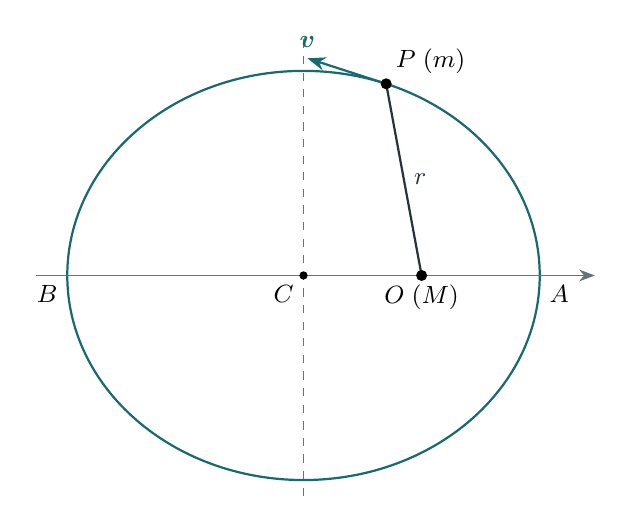
\begin{tikzpicture}[scale=1]
\draw[traj] (0.0000,0.0000) ellipse (3.0000 and 2.5981);

\coordinate (O) at (1.5,0);\coordinate (C) at (0,0);
\coordinate (P) at (1.05,2.434);\coordinate (A) at (3,0);\coordinate (B) at (-3,0);
\draw[axis] (-3.4,0)--(3.7,0);\draw[guide] (0,-2.8)--(0,3.0);
\draw[object] (O)--(P) node[midway,right] {$r$};
\draw[motion] (P)--++(-1.0,.324) node[above] {$\vect v$};
\fill (O) circle (2pt) node[below] {$O\;(M)$};\fill (C) circle (1.5pt) node[below left] {$C$};
\fill (P) circle (2pt) node[above right] {$P\;(m)$};
\node[below right] at (A) {$A$};\node[below left] at (B) {$B$};

\end{tikzpicture}
\figcaption{图 4.1　太阳位于焦点 $O$，椭圆中心为 $C$。}
\end{minipage}\par\medskip

\workarea

\clearpage

\pdfbookmark[2]{第 2 题 椭圆轨道反推平方反比引力}{q2}

\section*{第 2 题\quad 椭圆轨道反推平方反比引力}

\tagline{M-04-02}

已知行星沿椭圆轨道运动，太阳位于一个焦点，且径矢在相等时间内扫过相等面积。轨道的焦点极坐标方程为
\[
r=\frac{p}{1+e\cos\varphi},\qquad 0\leq e<1.
\]
试证明行星所受的力指向太阳，且大小与距离平方成反比。说明面积定律在证明中的作用，以及仅有轨道形状是否足够。

\par\medskip\noindent\begin{minipage}{\linewidth}\centering
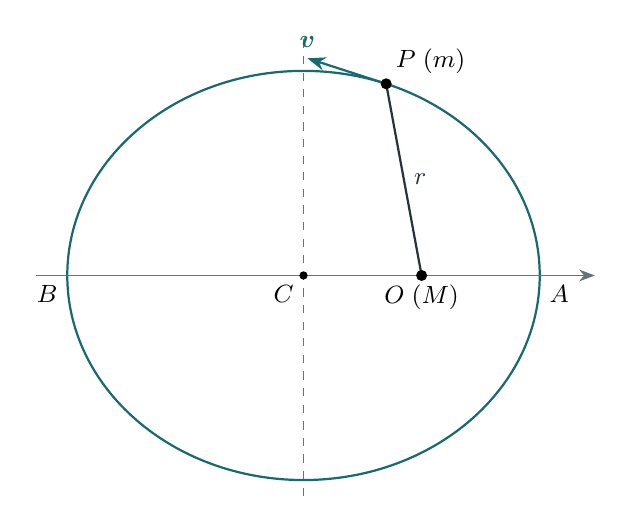
\begin{tikzpicture}[scale=1]
\draw[traj] (0.0000,0.0000) ellipse (3.0000 and 2.5981);

\coordinate (O) at (1.5,0);\coordinate (C) at (0,0);
\coordinate (P) at (1.05,2.434);\coordinate (A) at (3,0);\coordinate (B) at (-3,0);
\draw[axis] (-3.4,0)--(3.7,0);\draw[guide] (0,-2.8)--(0,3.0);
\draw[object] (O)--(P) node[midway,right] {$r$};
\draw[motion] (P)--++(-1.0,.324) node[above] {$\vect v$};
\fill (O) circle (2pt) node[below] {$O\;(M)$};\fill (C) circle (1.5pt) node[below left] {$C$};
\fill (P) circle (2pt) node[above right] {$P\;(m)$};
\node[below right] at (A) {$A$};\node[below left] at (B) {$B$};

\end{tikzpicture}
\figcaption{图 4.2　给定焦点椭圆及等面积时间规律。}
\end{minipage}\par\medskip

\workarea

\clearpage

\pdfbookmark[2]{第 3 题 初速度决定有心轨道类型}{q3}

\section*{第 3 题\quad 初速度决定有心轨道类型}

\tagline{M-04-03}

质量为 $M$ 的恒星固定不动，质量为 $m$ 的行星仅受其引力。行星位于距离 $r_0$ 处，初速 $v_0>0$ 与径矢垂直。讨论轨道为椭圆、圆、抛物线、双曲线时 $v_0$ 的取值，并指出椭圆情形下初始点是近点还是远点。另说明 $v_0=0$ 的退化情形。

\par\medskip\noindent\begin{minipage}{\linewidth}\centering
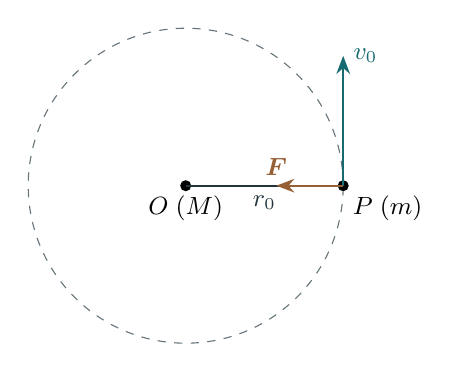
\begin{tikzpicture}[scale=1]

\draw[guide] (0,0) circle (2);\fill (0,0) circle (2pt) node[below] {$O\;(M)$};
\fill (2,0) circle (2pt) node[below right] {$P\;(m)$};
\draw[object] (0,0)--(2,0) node[midway,below] {$r_0$};
\draw[motion] (2,0)--(2,1.65) node[right] {$v_0$};
\draw[force] (2,0)--(1.15,0) node[above] {$\vect F$};

\end{tikzpicture}
\figcaption{图 4.3　初速度垂直于径矢；虚线圆用于比较轨道。}
\end{minipage}\par\medskip

\workarea

\clearpage

\pdfbookmark[2]{第 4 题 两质点万有引力相碰时间}{q4}

\section*{第 4 题\quad 两质点万有引力相碰时间}

\tagline{M-04-04}

空间中两质点质量分别为 $m_1,m_2$，仅以万有引力相互作用。开始时均静止，相距 $r_0$，随后相互靠近。求从释放到相碰所需的时间。按理想质点模型计算，相碰对应两者间距趋于零。

\par\medskip\noindent\begin{minipage}{\linewidth}\centering
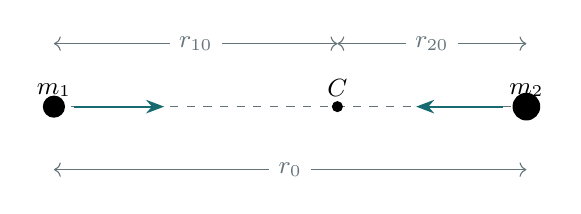
\begin{tikzpicture}[scale=1]

\draw[guide] (-3,0)--(3,0);\fill (-3,0) circle (4pt) node[above] {$m_1$};
\fill (3,0) circle (5pt) node[above] {$m_2$};\fill (.6,0) circle (2pt) node[above] {$C$};
\draw[motion] (-2.75,0)--(-1.6,0);\draw[motion] (2.7,0)--(1.6,0);
\draw[<->,muted] (-3,-.8)--(3,-.8) node[midway,fill=white] {$r_0$};
\draw[<->,muted] (-3,.8)--(.6,.8) node[midway,fill=white] {$r_{10}$};
\draw[<->,muted] (.6,.8)--(3,.8) node[midway,fill=white] {$r_{20}$};

\end{tikzpicture}
\figcaption{图 4.4　两质点同时向固定的质心 $C$ 运动。}
\end{minipage}\par\medskip

\workarea

\clearpage

\pdfbookmark[2]{第 5 题 绕月飞船两种登月喷气方案}{q5}

\section*{第 5 题\quad 绕月飞船两种登月喷气方案}

\tagline{M-04-05}

质量 $m=1.20\times10^4\,\mathrm{kg}$ 的飞船在月面上方 $h=100\,\mathrm{km}$ 的圆轨道运动。采用以下两种方式使轨道与月面相切：
\begin{enumerate}
\item 在 $A$ 向运动前方短时喷气，使飞船在 $B$ 与月面相切，$A,O,B$ 共线，$O$ 为月心。
\item 在 $A$ 沿径向向外短时喷气，使飞船在 $C$ 与月面相切，$OC\perp OA$。
\end{enumerate}
喷气相对飞船的速率恒为 $u=1.00\times10^4\,\mathrm{m/s}$；忽略喷气期间引力的冲量。月球半径 $R=1700\,\mathrm{km}$，月面重力加速度 $g=1.700\,\mathrm{m/s^2}$，月外引力遵从平方反比律。求两方案的速度改变量与燃料质量。月面相切只表示轨道到达条件，不包含软着陆制动。

\par\medskip\noindent\begin{minipage}{\linewidth}\centering
\begin{tikzpicture}[scale=.86]
\draw[object,fill=rulegray!25](0,0)circle(2.55);\draw[guide](0,0)circle(2.7);
\fill(0,0)circle(2pt);\node[below]at(0,0){$O$};
\fill(2.7,0)circle(2pt);\node[below right]at(2.7,0){$A$};
\draw[object](0,0)--(2.7,0)node[midway,below]{$R+h$};
\draw[motion](2.7,0)--(2.7,1.2)node[right]{$v_0$};
\fill(-2.55,0)circle(1.8pt);\node[left]at(-2.55,0){$B$};
\fill(0,2.55)circle(1.8pt);\node[above left]at(0,2.55){$C$};
\draw[guide](-2.55,0)--(0,0)--(0,2.55);\node at(-1,-1){月球};
\end{tikzpicture}
\figcaption{图4.5\quad 按$R:h=17:1$绘图；$B$、$C$分别是两种方案要求的月面相切点。}
\end{minipage}\par\medskip

\workarea

\clearpage

\pdfbookmark[2]{第 6 题 圆轨道径向脉冲后的近远地点}{q6}

\section*{第 6 题\quad 圆轨道径向脉冲后的近远地点}

\tagline{M-04-06}

飞船绕地球沿圆轨道运动，地面以上高度 $h=800\,\mathrm{km}$，地球半径 $R=6.40\times10^3\,\mathrm{km}$，圆轨道半径 $r_0=R+h$，速率 $v_0=3.00\times10^4\,\mathrm{km/h}$。短时沿径向向外喷气后，获得指向地心的径向速度 $v_r=800\,\mathrm{km/h}$，切向速度保持不变。忽略质量变化，求新椭圆轨道近地点、远地点距地面的高度。用题设圆轨道数据确定引力参数。

\par\medskip\noindent\begin{minipage}{\linewidth}\centering
\begin{tikzpicture}[scale=.84]
\draw[object,fill=rulegray!25](0,0)circle(2.666666667);
\draw[guide](0,0)circle(3);\draw[traj](0,-.080056929)ellipse(3.001067236 and 3.002134851);
\fill(0,0)circle(2pt);\node[below right]at(0,0){$O$};
\fill(3,0)circle(2pt);\node[below right]at(3,0){$P$};
\draw[object](0,0)--(3,0)node[midway,below]{$r_0$};
\draw[guide](3,0)--(3,1.4)node[right]{$v_0$};
\draw[motion](3,0)--(2.962666667,1.4)node[above left]{$\vect v_P$};
\draw[force](3,0)--(2.962666667,0);
\node[align=left,anchor=west]at(4,1.9){$v_r/v_0=2/75$\\向内径向分量很小};
\node at(-1,-1){地球};
\end{tikzpicture}
\figcaption{图4.6\quad 实际比例的轨道与速度分量；外虚圆是喷气前轨道，内圆是地表。}
\end{minipage}\par\medskip

\workarea

\clearpage

\pdfbookmark[2]{第 7 题 椭圆轨道发射探测器后的轨道}{q7}

\section*{第 7 题\quad 椭圆轨道发射探测器后的轨道}

\tagline{M-04-07}

飞船总质量为 $m$，其中探测器质量为 $m_0$。飞船绕质量 $M$ 的地球沿非圆椭圆运行，近地点距离为 $r_1$，速度为
\[
v_1=\sqrt{\frac{2\alpha GM}{r_1}}.
\]
\begin{enumerate}
\item 证明 $1/2<\alpha<1$，并求远地点距离 $r_2$ 与速度 $v_2$。
\item 在近地点沿运动方向发射探测器，使探测器进入抛物线轨道、剩余母船进入圆轨道。求 $m_0/m$ 及发射后探测器相对母船的速度 $u$。
\item 改在远地点，以同一质量比和同一相对速度 $u$ 向前发射，求探测器的新轨道，讨论其类型及发射点的性质。
\end{enumerate}
发射时间极短，忽略地球引力冲量及分离后二者间的引力。

\par\medskip\noindent\begin{minipage}{\linewidth}\centering
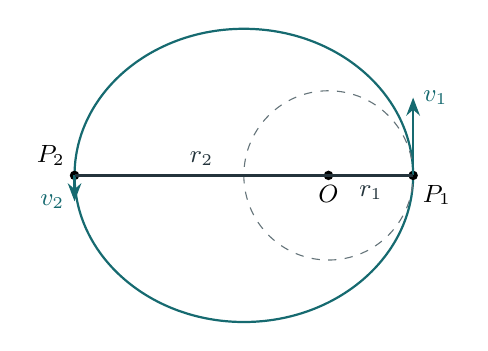
\begin{tikzpicture}[scale=0.86]
\draw[traj] (0.0000,0.0000) ellipse (2.5000 and 2.1651);
\draw[guide] (1.25,0) circle (1.25);
\fill (1.25,0) circle (2pt) node[below] {$O$};\fill (2.5,0) circle (2pt) node[below right] {$P_1$};
\fill (-2.5,0) circle (2pt) node[above left] {$P_2$};
\draw[motion] (2.5,0)--++(0,1.15) node[right] {$v_1$};
\draw[motion] (-2.5,0)--++(0,-.383333333) node[left] {$v_2$};
\draw[object] (1.25,0)--(2.5,0) node[midway,below] {$r_1$};
\draw[object] (1.25,0)--(-2.5,0) node[midway,above] {$r_2$};

\end{tikzpicture}
\figcaption{图 4.7　分别考虑在近地点 $P_1$、远地点 $P_2$ 向前发射。}
\end{minipage}\par\medskip

\workarea

\clearpage

\pdfbookmark[2]{第 8 题 彗星抛物线轨道与地球轨道交点}{q8}

\section*{第 8 题\quad 彗星抛物线轨道与地球轨道交点}

\tagline{M-04-08}

地球绕太阳沿半径 $R_0$ 的圆轨道运动，公转周期为 $T_E=1$ 地球年。彗星沿以太阳为焦点的抛物线运动，抛物线与地球轨道相交于一直径的两端。忽略地球与彗星间的引力。
\begin{enumerate}
\item 取太阳为原点、抛物线轴为 $y$ 轴，求极坐标和直角坐标轨道方程。
\item 求彗星最大速率与地球公转速率之比。
\item 求彗星在地球轨道内部运行的时间，以地球年表示。
\end{enumerate}

\par\medskip\noindent\begin{minipage}{\linewidth}\centering
\begin{tikzpicture}[scale=1]
\draw[guide] (0,0) circle (2);\draw[axis] (-2.6,0)--(2.8,0) node[right] {$x$};
\draw[axis] (0,-2)--(0,2.55) node[above] {$y$};
\draw[traj] plot[domain=-3:3,samples=70] (\x,{1-\x*\x/4});
\fill (0,0) circle (2pt) node[below left] {$O$};\fill (-2,0) circle (2pt) node[below left] {$A$};
\fill (2,0) circle (2pt) node[below right] {$B$};\fill (0,1) circle (2pt) node[above right] {$P$};
\node[above left] at (-1.4,1.6) {地球轨道};
\node[below] at (0,-2.45) {$OA=OB=R_0$};
\end{tikzpicture}
\figcaption{图 4.8　太阳在抛物线焦点 $O$，两交点为直径端点 $A,B$。}
\end{minipage}\par\medskip

\workarea

\clearpage

\pdfbookmark[2]{第 9 题 宇航站发射飞船后的再次相遇}{q9}

\section*{第 9 题\quad 宇航站发射飞船后的再次相遇}

\tagline{M-04-09}

质量为 $M$ 的宇航站与质量为 $m$ 的对接飞船一起绕地球沿半径 $nR$ 的圆轨道运动，$n=1.25$，$R$ 为地球半径。宇航站在 $A$ 将飞船沿原运动方向瞬时发射。发射后双方同向沿各自的椭圆轨道运行，飞船远地点距离为 $8nR$；宇航站质量仍为 $M$，忽略推进剂损失。

求质量比 $m/M$，使飞船运行一整周回到 $A$ 时恰与宇航站重新相遇。要求宇航站的整个轨道在地球表面之外，分离后忽略双方相互作用。

\par\medskip\noindent\begin{minipage}{\linewidth}\centering
\begin{tikzpicture}[scale=.96]
\draw[object,fill=rulegray!25](0,0)circle(.56);
\draw[guide](0,0)circle(.7);
\draw[traj](-2.45,0)ellipse(3.15 and 1.979898987);
\draw[object](.02135307264,0)ellipse(.67864692736 and .678310915660);
\fill(0,0)circle(1.7pt)node[below]{$O$};
\fill(.7,0)circle(2pt)node[below right]{$A$};
\fill(-5.6,0)circle(2pt)node[below]{$B$};
\fill(-.657293855,0)circle(1.7pt)node[above left]{$P_s$};
\node at(-2.5,2.4){飞船轨道};
\node[anchor=west]at(1.65,-1.05){宇航站轨道};
\draw[guide](1.65,-.95)--(.35,-.57);
\draw[motion](.7,0)--(.7,1.4)node[above]{$v$};
\draw[motion](1.35,0)--(1.35,1.033349281)node[above right]{$v'$};
\draw[guide](.7,0)--(1.35,0);
\node[anchor=west,align=left]at(1.8,.2){$k=10$\\地球半径$R$};
\end{tikzpicture}
\figcaption{图4.9\quad 以$k=10$的可行轨道示意；$A$是飞船近点、宇航站远点。}\end{minipage}\par\medskip

\workarea

\clearpage

\pdfbookmark[2]{第 10 题 地火霍曼转移轨道}{q10}

\section*{第 10 题\quad 地火霍曼转移轨道}

\tagline{M-04-10}

地球、火星同向沿半径分别为 $r_E,r_M$ 的圆轨道绕太阳运动，$r_M>r_E$。火箭离地后进入日心转移椭圆，近日点在地球轨道，远日点在火星轨道；发射速度方向与地球公转速度方向相同，并选择发射时机使火箭到达远日点时遇到火星。只计太阳引力，太阳质量为 $M_S$。
\begin{enumerate}
\item 火箭进入日心转移轨道时，相对地球需有多大速度？
\item 从出发到到达火星需多久？用地球公转周期 $T_E=1$ 年表示。
\end{enumerate}
这里的相对速度在忽略地球引力的模型中定义；若从地面实际发射，还需另外处理脱离地球引力的过程。

\par\medskip\noindent\begin{minipage}{\linewidth}\centering
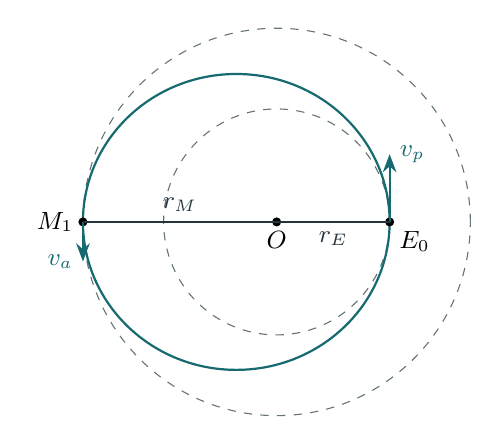
\begin{tikzpicture}[scale=.82]
\draw[guide](0,0)circle(1.75);\draw[guide](0,0)circle(3);
\draw[traj](-.625,0)ellipse(2.375 and 2.291287847);
\fill(0,0)circle(2pt)node[below]{$O$};
\fill(1.75,0)circle(2pt)node[below right]{$E_0$};
\fill(-3,0)circle(2pt)node[left]{$M_1$};
\draw[motion](1.75,0)--(1.75,1.05)node[right]{$v_p$};
\draw[motion](-3,0)--(-3,-.6125)node[left]{$v_a$};
\draw[object](0,0)--(1.75,0)node[midway,below]{$r_E$};
\draw[object](0,0)--(-3,0)node[midway,above]{$r_M$};
\end{tikzpicture}
\figcaption{图4.10\quad 转移椭圆在$E_0$、$M_1$处与两圆轨道相切；速度箭头符合角动量守恒。}\end{minipage}\par\medskip

\workarea

\clearpage

\pdfbookmark[2]{第 11 题 火星圆轨道径向微扰后的椭圆轨道}{q11}

\section*{第 11 题\quad 火星圆轨道径向微扰后的椭圆轨道}

\tagline{M-04-11}

飞船以速率 $v_0$ 绕火星沿圆轨道运动。火星半径 $R$，原轨道高度 $H$，$r_0=R+H$。飞船短时沿径向向外喷气，获得指向火星的速度 $\alpha v_0$，其中 $0<\alpha\ll1$；切向速度不变，质量变化可忽略。
\begin{enumerate}
\item 求新椭圆近火点、远火点距火星表面的高度 $h_A,h_B$。
\item 求新轨道周期，并讨论与原周期相比从哪一阶开始改变。
\end{enumerate}
同时检查新轨道是否触及火星表面。

\par\medskip\noindent\begin{minipage}{\linewidth}\centering
\begin{tikzpicture}[scale=.85]
\draw[object,fill=rulegray!25](0,0)circle(1.9);
\draw[guide](0,0)circle(2.35);
\draw[traj](0,-.117794486)ellipse(2.352943019 and 2.355889724);
\coordinate(O)at(0,0);\coordinate(P)at(2.35,0);
\draw[object](O)--(P)node[midway,below]{$r_0$};
\draw[guide](P)--++(0,1.2)node[right]{$v_0$};
\draw[force](P)--++(-.06,0);
\draw[motion](P)--++(-.06,1.2)node[above left]{$\vect v_P$};
\fill(O)circle(2pt)node[below right]{$O$};
\fill(P)circle(2pt)node[below right]{$P$};
\node[align=left,anchor=west]at(3,1.8){示例$\alpha=0.05$\\径向分量$-\alpha v_0$\\图中$H/R=9/38$};
\end{tikzpicture}
\figcaption{图4.11\quad 圆轨道、脉冲及新椭圆使用同一参数；虚圆为喷气前轨道。}\end{minipage}\par\medskip

\workarea

\clearpage

\pdfbookmark[2]{第 12 题 借助火星引力弹弓逃离太阳系}{q12}

\section*{第 12 题\quad 借助火星引力弹弓逃离太阳系}

\tagline{M-04-12}

从地面发射飞船逃离太阳系，考虑两种方案：一是直接获得足够的日心能量；二是先到火星附近，借助其引力偏转后逃离。地球、火星在同一平面同向作日心圆周运动，忽略空气阻力和地球自转。
\begin{enumerate}
\item 直接逃逸时，求最小地面发射速率 $v_a$ 及离地余速的最有利方向。
\item 沿该方向发射，地面速率为 $v_b$。在火星尚远、可忽略其引力时，求飞船穿过火星轨道的日心切向分量 $v_\parallel$ 和向外径向分量 $v_\perp$。
\item 若借火星引力使飞船离开火星时沿火星公转方向运动，求能逃离太阳的最小地面发射速率。
\item 比较两方案的地面发射动能，求理想情况下最多节约的百分比。
\end{enumerate}
数据：地球公转速率 $v_E=30\,\mathrm{km/s}$，$r_E:r_M=2:3$，地球半径 $R_E=6400\,\mathrm{km}$，地面 $g=9.80\,\mathrm{m/s^2}$。采用分段二体近似：地球附近用地心系、两行星间用日心系、火星附近用火星系。本题理想偏转模型不限制火星的半径及最大可实现偏转角；须说明这个条件对节能上限的意义。

\par\medskip\noindent\begin{minipage}{\linewidth}\centering
\begin{tikzpicture}[scale=.93]
\pgfmathsetmacro{\velx}{1.1851728543457754}
\pgfmathsetmacro{\pin}{\velx*\velx}
\pgfmathsetmacro{\ein}{\pin-1}
\pgfmathsetmacro{\fm}{acos((2*\pin/3-1)/\ein)}
\draw[guide](0,0)circle(1.7);\draw[guide](0,0)circle(2.55);
\draw[traj,domain=0:\fm,samples=90]
plot({1.7*\pin*cos(\x)/(1+\ein*cos(\x))},{1.7*\pin*sin(\x)/(1+\ein*cos(\x))});
\draw[motion,domain=\fm:155,samples=70]
plot({5.1*cos(\x)/(1+cos(\x-\fm))},{5.1*sin(\x)/(1+cos(\x-\fm))});
\fill(0,0)circle(2pt)node[below]{太阳$O$};
\fill(1.7,0)circle(2pt)node[below right]{地球（出发时）};
\fill({2.55*cos(\fm)},{2.55*sin(\fm)})circle(2pt)node[above right]{火星（遭遇时）};
\draw[motion](1.7,0)--++(0,1.1)node[right]{$\vect V$};
\draw[object](0,0)--({2.55*cos(\fm)},{2.55*sin(\fm)});
\node[anchor=west]at(1.9,-1.5){$r_E:r_M=2:3$};
\end{tikzpicture}
\figcaption{图4.12\quad 辅助方案按临界速度的日心入射椭圆及出射抛物线绘制，火星近区以短程拼接表示。}
\end{minipage}\par\medskip

\workarea

\clearpage

\pdfbookmark[2]{第 13 题 弹簧有心力场中的有效势能曲线}{q13}

\section*{第 13 题\quad 弹簧有心力场中的有效势能曲线}

\tagline{M-04-13}

劲度系数 $k=3.0\,\mathrm{N/m}$ 的弹簧一端固定于 $O$，另一端连接质量 $m=2.0\,\mathrm{kg}$ 的质点。质点在光滑水平面内绕 $O$ 作匀速圆周运动，总机械能 $E_0=12\,\mathrm J$。忽略弹簧原长。突然给质点径向一击，使其获得向外速度 $v_{r0}=1.0\,\mathrm{m/s}$。
\begin{enumerate}
\item 用有效势能曲线描述打击前、后的运动，画出真实势能、角动量项及两条总能量线。
\item 求打击后的半径范围，并说明转折点的速度是否为零。
\end{enumerate}

\par\medskip\noindent\begin{minipage}{\linewidth}\centering
\begin{tikzpicture}[scale=1]

\draw[guide] (0,0) circle (2);\fill (0,0) circle (2pt) node[below] {$O$};
\draw[decorate,decoration={zigzag,segment length=4mm,amplitude=1.4mm}] (0,0)--(2,0);
\fill (2,0) circle (3pt) node[below right] {$P\;(m)$};
\draw[motion] (2,0)--(2,1.15) node[right] {$v_0$};
\draw[force] (2,0)--(2.469485534,0) node[right=3pt] {$v_{r0}$};
\node at (-1.4,2.45) {光滑水平面};

\end{tikzpicture}
\figcaption{图 4.13　原长忽略的弹簧与新增向外径向速度。}
\end{minipage}\par\medskip

\workarea

\clearpage

\pdfbookmark[2]{第 14 题 均匀宇宙尘埃中的圆形行星轨道}{q14}

\section*{第 14 题\quad 均匀宇宙尘埃中的圆形行星轨道}

\tagline{M-04-14}

质量 $m$ 的行星绕固定质量 $M$ 的恒星运动。恒星周围球对称地分布着均匀、稀薄尘埃，密度为 $\rho$。尘埃分布覆盖所研究轨道及其小扰动范围，直接碰撞可忽略；行星只受恒星与尘埃的引力。
\begin{enumerate}
\item 角动量为 $L>0$ 的圆轨道半径 $r_0$ 满足什么方程？列出即可。
\item 研究该圆轨道的小径向偏离，解释轨道可近似看作缓慢进动的近圆椭圆；证明进动方向与公转方向相反，并求进动角速度。
\end{enumerate}
取公转方向为正。要求区分小径向偏离的一阶近似与尘埃密度很小时的进一步展开。

\par\medskip\noindent\begin{minipage}{\linewidth}\centering
\begin{tikzpicture}[scale=1]
\draw[object] (0,0) circle (2.5);\fill[accent!10] (0,0) circle (2.5);
\draw[guide] (0,0) circle (1.6);\fill (0,0) circle (3pt) node[below] {$M$};
\fill (1.6,0) circle (2pt) node[below right] {$m$};\draw[motion] (1.6,0)--(1.6,1.0) node[right] {$v_0$};
\draw[object] (0,0)--(1.6,0) node[midway,below] {$r_0$};\node at (-1.3,1.7) {$\rho$ 均匀};

\end{tikzpicture}
\figcaption{图 4.14　尘埃球对称分布，外层球壳对行星的合引力为零。}
\end{minipage}\par\medskip

\workarea

\end{document}
